\chapter{Software Defined Radio}
\label{chap:sdr}

\section{Overview}%ok
\label{sdr:overview}

In the modern world everything is becoming "smarter", and the cloud paradigm is
creating a new way to organize the infrastructure, so telecommunications will
also be affected by such changes. For example, the RAN as a service  paradigm
and cloud requires devices which are both scalable and reconfigurable following
customer demands. To accomplish that, there are some schemes and theories
involved, but this work will focus on a device that fits in the \emph{Software
Defined Radio} scope, which is defined according to the \emph{SDR Forum}
\cite{web:sdrforum} as:\\

\begin{displayquote}
\textit{Radios that provide software control of a variety of modulation techniques,
wide-band or narrow-band operation, communications security functions (such as
hopping), and waveform requirements of current \& evolving standards over a
broad frequency range.}\\
\rightline{{\textit{SDR Forum} \cite{web:sdrforum}}}
\end{displayquote}

In short, \textit{Software-Defined Radio} (SDR) refers to the technology wherein
software modules running on a generic hardware platform consisting of DSPs, FPGA
and general purpose microprocessors are used to implement radio functions which
previously where implemented only in analog hardware, and recently could be
implemented in software due to the evolution of programmable devices. One
example is generation of signals at the transmitter and tuning/detection of
received radio signal (demodulation) at receiver.

This is a very powerful concept and it has been idealized over 20 years ago
\cite{ladimer2009}. However, after the 2000's the DSP and FPGA technology
improved and its implementation became feasible \cite{ladimer2009}. SDR has some
very interesting applications, in this chapter the educational and
telecommunications applications of SDR shall be explored.

SDR is a very elastic platform but its use is not recommended in every
situation. This is because of the cost necessary to implement SDR, which incites
our question: \emph{what is the real advantage in SDR?} According to worldwide
telecommunication reports and works \cite{introlte}, every time a standard is
changed there is a huge cost of buying new equipment capable of handling the new
standard by both user and operator so SDR tries to reduce these costs by
maintaining legacy systems while being able to upgrade to newer
systems \cite{dayananda2012}. This fact generated a lot of interest in SDR by the
wireless communication industry because of the economic advantages it could
bring. Another great advantage for companies to implement SDR is that they can
use the same hardware and this hardware would work in all communication schemes
around the world regardless of any regulations that would otherwise require
transceiver variations for certain markets.

% The use of SDR is growing in the industry and seems to be a promise for the
%Cloud-RAN environment, where radio infrastructure would adapt itself to the
%customer needs.

\section{Cloud Computing Overview}
\label{sec:sdr_cloud}

Cloud computing is a computing paradigm, where a large variety of systems are
connected through networks, being able to provide dynamically scalable
infrastructure for application, data and file storage. With the advent of this
technology, the cost of computation resources, application hosting, content
storage and delivery is reduced significantly.

%Cloud computing is a practical approach to experience direct cost benefits and
%it has the potential to transform a data center from a capital-intensive set up
%to a variable priced environment. \\

The idea of cloud computing is based on a very fundamental principle of
\emph{reusability of IT resources}. The difference that cloud computing brings
compared to traditional concepts of "grid computing", "distributed computing",
"utility computing", or "autonomic computing" is to broaden horizons across
organizational boundaries.

There are three main types of cloud in current use:

\begin{itemize}

    \item \textbf{Infrastructure as a Service (IaaS):} offers managed and
    scalable resources as services to the user, by enhancing virtualization
    capabilities. Servers, storage systems, switches, routers, and other systems
    are pooled and made available to handle workloads that range from
    application components to high-performance computing applications. For 5G
    there is the idea to implement RAN as a Service or C-RAN, meaning that all
    the telecommunication devices can be used on an on-demand basis by
    costumers. The user do not need to worry about maintenance of the hardware
    system, reducing information technology professional (IT) costs.

    \item \textbf{Platform as a Service (PaaS):} avails computational resources
    via a platform upon which applications and services can be developed and
    hosted. \textit{PaaS} typically makes use of dedicated \textit{APIs} to
    control the behavior of a server hosting engine which executes and
    replicates the execution according to user requests. In short \textit{PaaS}
    enables the user to develop and host the application on the cloud without
    the need to worry with all the infrastructure to run it. However this
    service is limited to a specific \textit{API} or Environment.

    \item \textbf{Software as a Service (SaaS):} features a complete application
    offered as a service on demand. A single instance of the software runs on the
    cloud and services multiple end users or client organizations.

\end{itemize}

\section{GNUradio}
\label{sdr:gnuradio}

When SDR is mentioned the first thing that comes in mind is GNUradio, because it
is a Open Source Software widely used in academic environment to teach and
research Software-defined Radios and implement very interesting applications. It
is widely used in radio amateur, academic and commercial environments to support
both wireless communications research and real-world radio systems. Furthermore,
it can be used both with low cost external RF hardware to implement SDR and it
can be used as a simulation environment with \textit{GNUradio companion}.
GNUradio Companion is a graphical interface to help visualize the system in
block-diagram fashion.

When coupled to an analog front-end such as the one used in this work, GNU Radio
can be used to perform all the baseband signal processing. It is possible write
applications to receive data out of digital streams or to push data into digital
streams, which is then transmitted using hardware known as \textit{Universal
Software Radio Peripheral} (USRP). GNU Radio has filters, channel encoders,
synchronization elements, equalizers, demodulators, vocoders, decoders, and many
other elements. Furthermore, extending GNU Radio is straightforward, because
everything is modular, if there is need for a block, it is just a matter of
following the conventions and the block can easily fit in the system.

Since GNU Radio is a software, it can only handle digital data. Usually, complex
baseband samples, better know as IQ samples, which are the input data type for
receivers and the output data type for transmitters. Analog hardware is then
used to shift the signal to the desired carrier frequency. That requirement
aside, any data type can be passed from one block to another - be it bits,
bytes, vectors, bursts or more complex data types.

GNU Radio applications are primarily written using the Python programming
language, while the supplied, performance-critical signal processing path is
implemented in C++ using processor floating point extensions, where available.

USRP stands for Universal Software Radio Peripheral, which is basically an FPGA
connected to a transceiver that allows the systems made inside the GNUradio
software to be implemented in real-world, it means that USRP is a hardware for
implementing Software Radios.

In Figure \ref{fig:usrpbd} there is the block diagram of a comercial USRP
model (N210), which is composed by Ethernet PHY and USRP Hardware Driver (UHD)
protocol command and control for data input and output via Ethernet. The
transmission and reception is made by the daughter board, which is usually a
transceiver, for this the USRP must be equiped with decimator block in the receiver path to
from Analog to Digital Converter (ADC) and an interpolator block in the transmitter path to the
Digital to Analog Converter (DAC). All the control and configuration is done by
a RISC processor which has the role of initializing the peripherals and configuring
them. The last thing necessary to transmission is a clock source and in this
Figure \ref{fig:usrpbd} there is the possibility to have an external reference
clock, which is very interesting for critical systems.

%usrp n210 block diagram
\begin{figure}[htbp]
    \centering
    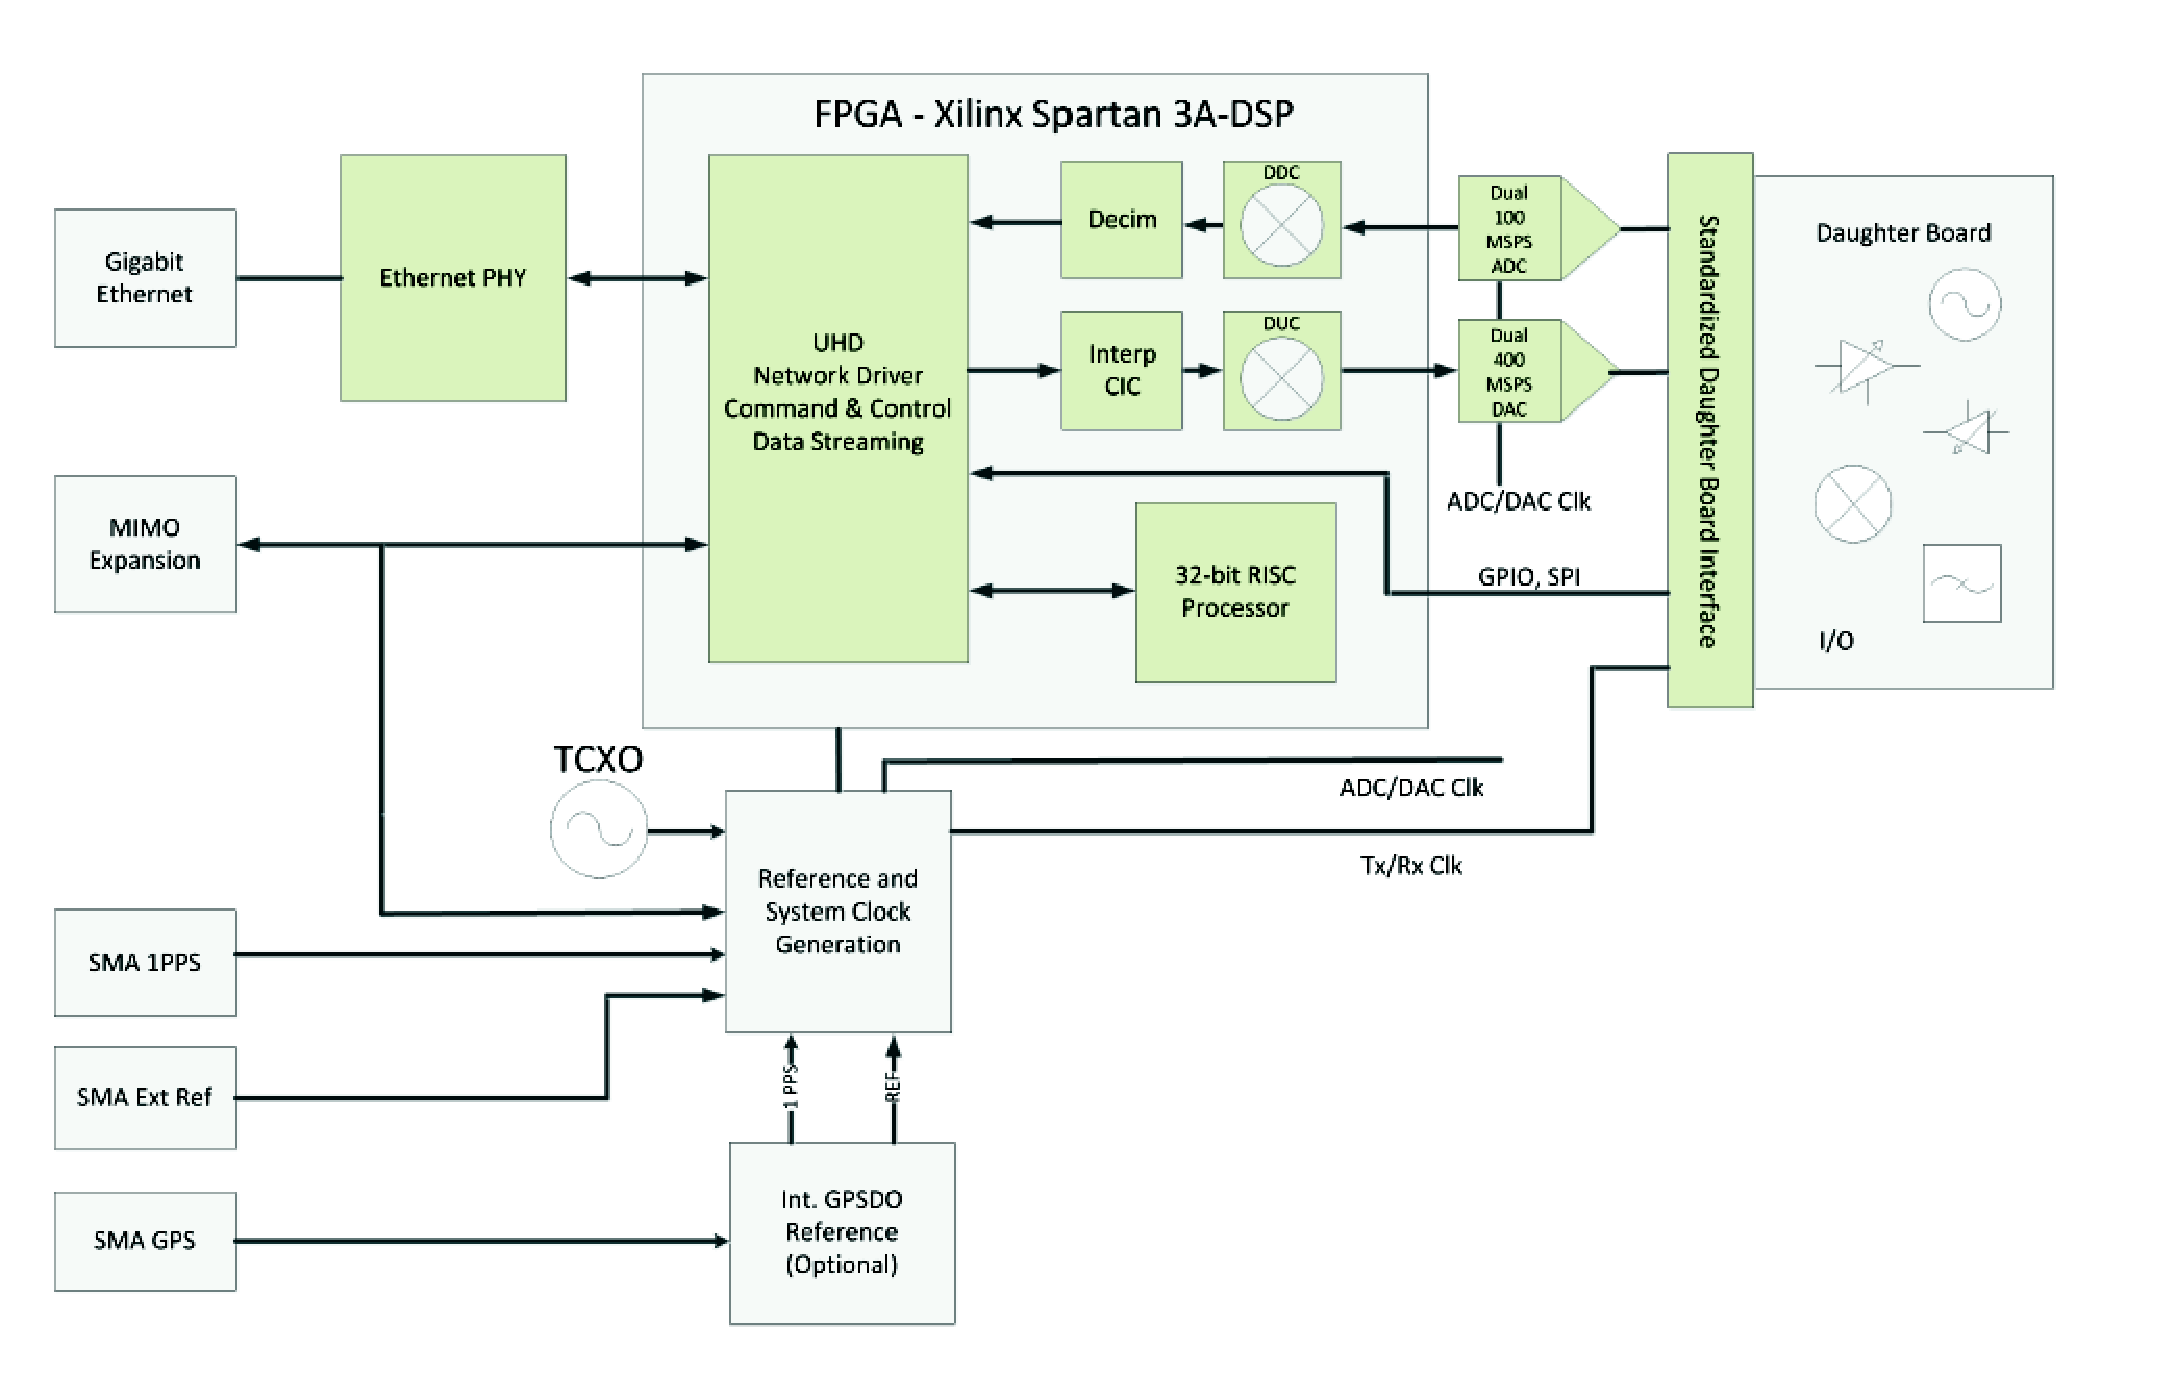
\includegraphics[width=.85\textwidth]{./figures/usrp_bd}
    \caption{ USRP N2010 block diagram.
    \label{fig:usrpbd}}
\end{figure}

The USRP communicates with the computer by the UHD protocol, and GNUradio
automatically recognizes it, making possible to send and receive signals in the
desired frequency. With UHD GNUradio software can read and write in the USRP
from both USB and ETHERNET connection, which makes easy to implement the
generated digital system in a real communication system. USRP is not a hardware
exclusive to GNUradio, there are other communications engineering softwares
which are able to use such hardware, such as \textit{Mathwork's Simulink}.

\section{SDR Applications in C-RAN}
\label{sec:sdr_app}

As stated before in Section \ref{sdr:overview}, SDR has a wide range of applications,
and very interesting advantages over the current systems. This section shall focus
on the C-RAN applications of \emph{Software-defined Radio}.

C-RAN comes from the cloud idea of Infrastructure as a service (IaaS) or in this
case RAN as a service, thus it needs a reconfigurable and scalable
infrastructure to fulfill the customer needs. SDR is perfect for such
applications because  it is in essence reconfigurable and scalable.

The two images below contrast the past RAN infrastructure in Figure
\ref{fig:tran}, where there is a baseband processing unit on every transmission
tower, increasing the costs of maintenance and deployment. The traditional RAN
scheme is still in use today. However, it is not economically or technologically
interesting, that is were C-RAN paradigm in Figure \ref{fig:cran} aims to
change, with it all the processing elements of the systems are centralized in a
server-farm like disposition and the radio front-haul can be dynamically used
depending on the needs of the network. Thus there is the need of reconfigurable
and scalable front-haul infrastructure.


%RAN network image
\begin{figure}[htbp]
    \centering
    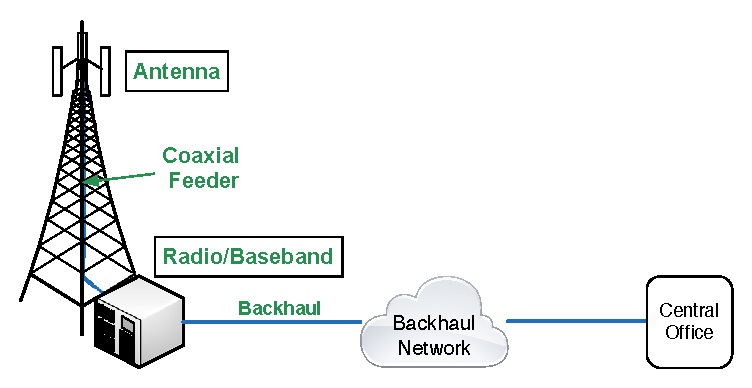
\includegraphics[width=0.65\textwidth]{./figures/traditional_bs}
    \caption{ Traditional Radio Access Netwok
    \label{fig:tran}}
\end{figure}

%C-RAN network image
\begin{figure}[htbp]
    \centering
    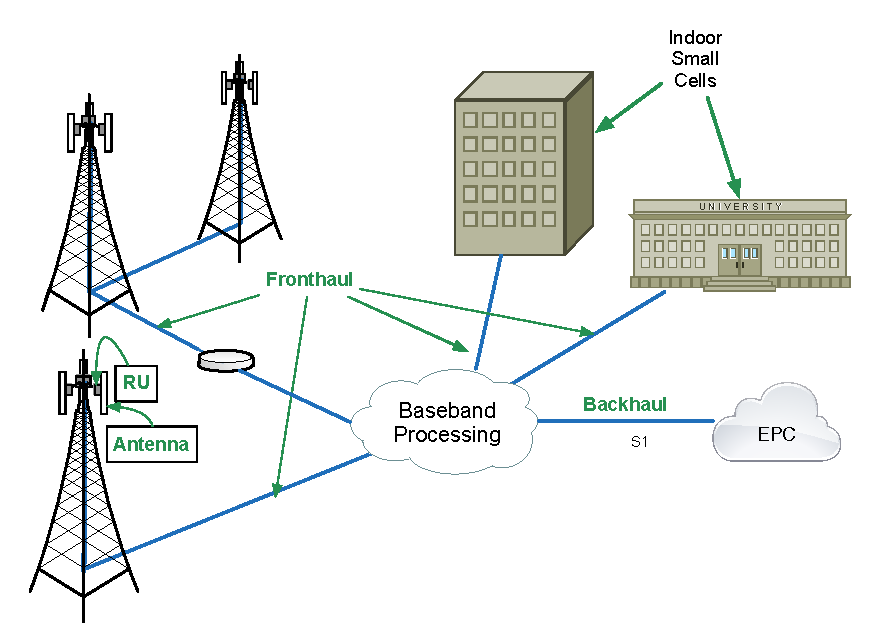
\includegraphics[width=0.65\textwidth]{./figures/c_RAN}
    \caption{ Centralized RAN paradigm.
    \label{fig:cran}}
\end{figure}

There are many works in SDR for modern communication schemes being done in
recent years, and before the concept of C-RAN was a buzz the academy began to
think how to control SDR in cloud environments \cite{dayananda2012}. Other
works were focusing on transmitting on the GHz frequency band of the modern
communications schemes (3GPP, LTE) \cite{kelley2009} and \cite{neenu2014}.

Since the same hardware is used to implement various telecommunications schemes,
the main advantages of the use of SDR in C-RAN environment, according to
\cite{dayananda2012} are the reduction of the costs for the network operators in
terms of maintaining the legacy systems while changing standards, reduced
maintenance cost and remote control. For the end user the cost reduction is
passed to cheaper roaming.

\section{Educational Applications of SDR}

In the educational environment SDR brings real-world conditions to the lab. The
student or researcher can experiment in a myriad of configurations and make
tests in the real-world channels instead of just simulating. However, this is
only possible with a hardware implementation of the SDR, there are software
implementations which use computer sound card ADC and DAC to communicate on
voice range frequencies \cite{ladimer2009}.

Having a testbed or simulation to apply all the knowledge acquired in classroom
is crucial to engineering courses. The engineering students often get bored easy
by all the theoretical study and prefer to learn by practice, thus SDR is a
suitable platform to teach digital signal processing, digital communications and
any course related to those subjects.

A very famous setup for academic and research in SDR is the duo GNUradio
\cite{web:gnuradio} and USRP \cite{web:usrp} mentioned in the previous section
\ref{sdr:gnuradio} which can easily implement a communication system with drag
and drop graphical interface. In \cite{akbook} there is some stimulus to work
with GNUradio.


\section{Implementations}
\label{sdr:implement}

Software defined radio implementations vary widely depending on available
equipment or standard to be implemented. According to \cite{ladimer2009}, the basic
architecture of SDR is composed by filters, analog to digital converters (ADC),
digital to analog converters (DAC) and a processor in the core of the system
which could be implemented using DSP for example.

\begin{figure}[htbp]
    \centering
    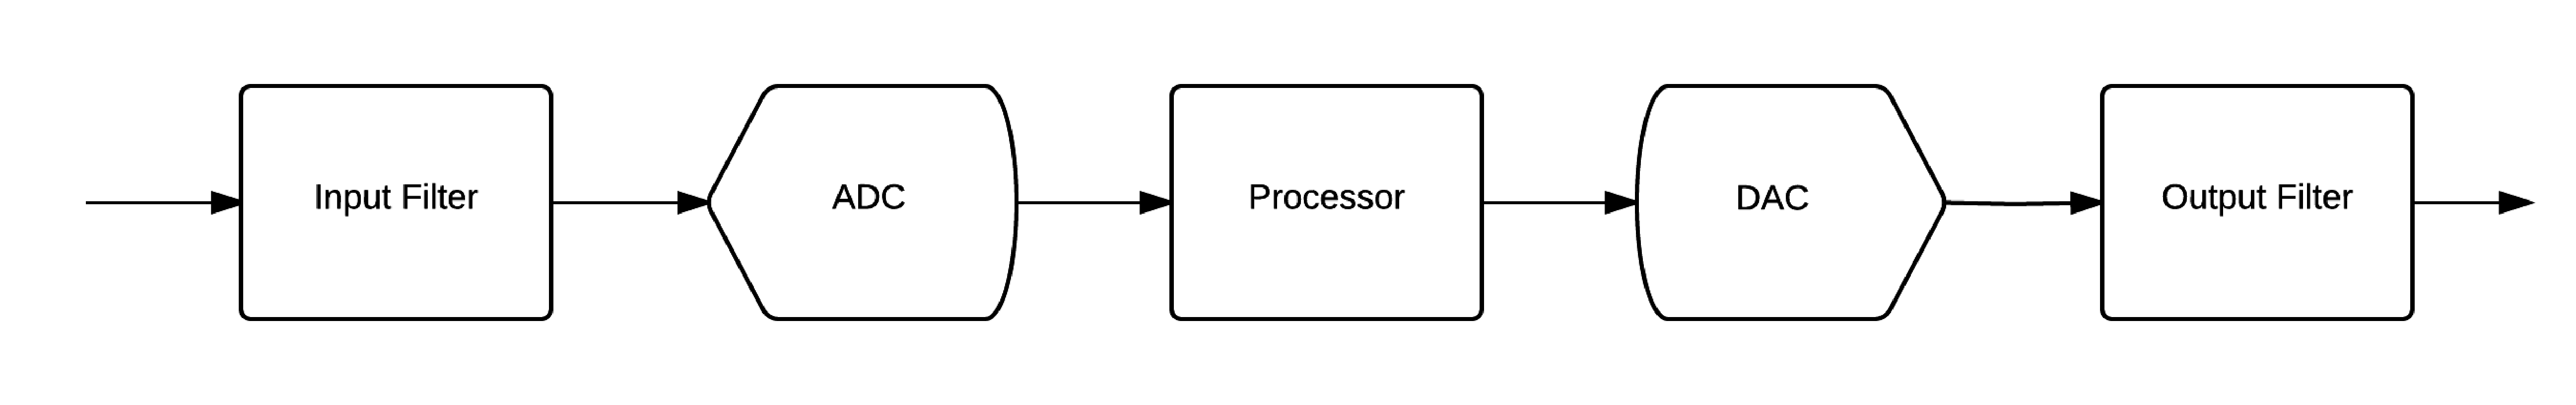
\includegraphics[width=0.8\textwidth]{./figures/sdr_basic_arch}
    \caption{ Software defined radio basic architecture.
    \label{fig:sdr_basic}}
\end{figure}


Implementations may vary a lot, some common implementations are done in
\textit{Mathwork's Simulink} and use the computer’s sound card as a
communication channel. A more difficult but more interesting implementation
involves the use of DSP chips to implement the signal processing functions and
some ADC and DAC chips can compose the SDR system.

In addition to DSP cores and ADC/DAC integrated circuits, every SDR prototype
must be featured with proper antennas. The latter, in particular, must be
chosen according to the desired transmission bandwidth.

This work has a SDR like implementation done in FPGA and using the transceiver
AD9361 which makes upconversion (transmitter) and downconversion
(receiver), filters and make analog to digital conversion and digital to analog
conversion. It is possible to implement transmitter and receiver with only
one board.
%However the most complex part does not lie in the system itself
%because some electronic parts became a commodity, the complexity is in the
%modulation/demodulation blocks and all the synchronization process, such topics
%shall be discussed in the chapter \ref{chap:lte}.
